\newpage
\section{Aufgabe 1}
Machen Sie Sich vertraut mit der Verwendung der Wire Libarary für TWI/I2C zur Kommunikation zwischen Geräten (\url{http://energia.nu/reference/wire/}).\\
Lesen Sie das Datenblatt zum integrierten Schaltkreis DS1621:\\
\url{http://pdfserv.maximintegrated.com/en/ds/DS1621.pdf}. Der DS1621 ist ein digitales Thermometer mit einer TWI-Schnittstelle. Betrachten Sie im Folgenden das Schaltbild 5. Die Pins 5, 6 und 7 des DS1621 sind mit der Masse verbunden. Das Launchpad ist über die Pins PB\_2 (SCL) und PB\_3 (SDA) verbunden. Das Launchpad agiert als Master, der DS1621 als Slave.
\begin{figure}[h]
	\centering
	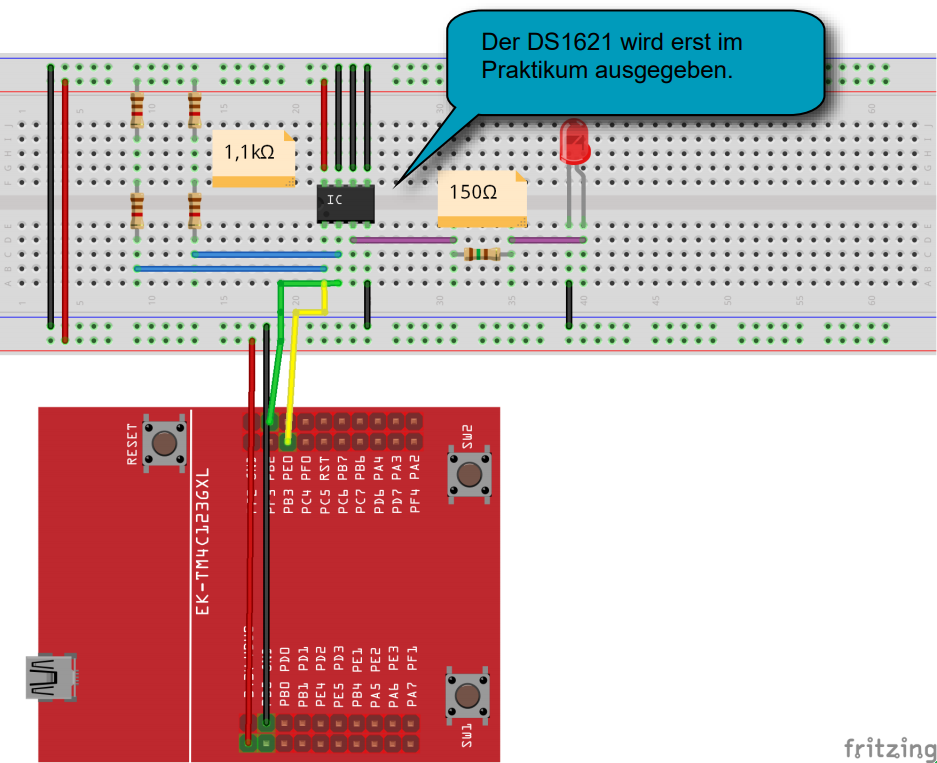
\includegraphics[width=0.7\linewidth]{images/Schaltplan5}
	\label{fig:Schaltplan5}
\end{figure}
\begin{center}
	Schaltplan 5
\end{center}
Beantworten Sie die Fragen vor dem Praktikum schriftlich:
\subsection{Aufgabe 1a}
Wie lautet die Adresse das DS1621, mit dem dieser in der dargestellten Schaltung angesteuert wird? Erklären Sie, wie sich die Adresse zusammensetzt und wie Sie die Adresse mit der Wire-Bibliothek benutzen.
\begin{figure}[h!]
\centering
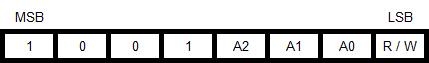
\includegraphics[width=0.7\linewidth]{images/SlaveAdresse}
\label{fig:SlaveAdresse}
\end{figure}

\noindent Die Adresse ist 7 Bit gor\ss{}. Das Achte bzw. das LSB ist das Lese/Schreib-Bit. Die ersten vier Bits sind mit dem Wert $"$1001$"$ gesetzt. Die nächsten drei Bits werden mit den Adress-Pins A2, A1, A0 (Pin 5 - 7) gesetzt. Da alle Adress-Pins mit der Masse verbunden sind lautet die Adresse $"$1001000$"$.\\
Die Methoden \textit{Wire.begin()}, \textit{Wire.requestFrom()} und \textit{Wire.beginTransmission()} haben die Adresse als Parameter.
\subsection{Aufgabe 1b}
Wie setzt sich das Format zur Übertragung von Temperaturwerten bei dem DS1621 zusammen? Welche Befehle und Parameter (mit der Wire-Bibliothek) müssen an den DS1621 gesendet werden, um dessen Pin 3 ($T_{OUT}$) so einstellen, dass dieser bei einer Temperatur grö\ss{}er 25\textdegree{} Celsius auf HIGH geht?\\ \\
Die Temperatur wird mit 9-Bits codiert. Das hei\ss{}t es werden 2 Byte verwendet. Wenn das erste Bit (vom Ersten Byte) mit einer Eins gesetzt ist, ist die Temperatur negativ. Die nächsten 7 Bits codieren die Temperatur. Das erste Bit vom zweiten Byte codiert 0,5\textdegree{} Celsius. Die darauf folgenden Bits sind alle mit dem Wert 0 gesetzt.\\ \\
00011001 00000000 = +25\textdegree{}C\\
11100111 00000000 = -25\textdegree{}C\\
00000000 10000000 = +0,5\textdegree{}C\\
\begin{lstlisting}
//init
Wire.setModule(0);
Wire.begin();

Wire.beginTransmission(144); // 1001000
Wire.write(172);             // Access Config ACh
Wire.write(2);
Wire.endTransmission();
Wire.beginTransmission(144); // 1001000
Wire.write(161);             // Access TH A1h
Wire.write(25);              // 25 Grad Celsius
Wire.write(0);
Wire.endTransmission();
\end{lstlisting}
\subsection{Aufgabe 1c}
Mit welchen Anweisungen bekommen Sie die Temperatur vom DS1621 geliefert?
\begin{lstlisting}
//init
float t = 0;
Wire.setModule(0);
Wire.begin();

Wire.beginTransmission(145); // 1001000
Wire.write(170);             // Read Temperature AAh
Wire.endTransmission();

Wire.requestFrom(145, 2);
byte val = Wire.read();
if((val & 128) != 0) {
  t = val - 256;
} else {
  t = val;
}
val = Wire.read();
if(val != 0) {
  t += 0.5;
}
\end{lstlisting}
\section{Aufgabe 2}
Programmieren Sie das Launchpad bzw. den DS1621 in der oben gezeigten Schaltung dahingehend, dass der DS1621 kontinuierlich die aktuelle Umgebungstemperatur misst und das Launchpad diese über den serial Monitor ausgibt.\\ \\
Programmieren Sie die Schaltung so, dass beim Überschreiten einer einstellbaren Temperatur (z.B. 24\textdegree{}C) die LED an und beim Unterschreiten der Temperatur die LED ausgeht.\\ \\
\textbf{Tipp:} Sie können das Programm vorher schon vorbereiten und die Bearbeitungszeit nur für eventuelle Anpassungen nutzen.\\ \\
\textbf{Tipp:} Rufen Sie vor der Benutzung der Wire-Bibliothek die Methode\\
\textit{Wire.setModule(0)} auf, um das richtige $I^2C$-Modul des Launchpads auszuwählen.\\ \\
